% Set up the document twoside oneside
\documentclass[a4paper,12pt]{Thesis}  % Use the "Thesis" 
\graphicspath{Images/}  

%% Please keep all the figure inside the Figure folder. Location of the graphics files (set up for graphics to be in PDF format)


\usepackage{setspace}

% Include any extra LaTeX packages required
\usepackage[square, numbers, comma, sort&compress]{natbib}  % Use the "Natbib" style for the references in the Bibliography
%\usepackage{chapterbib}
%\usepackage[sectionbib]{chapterbib}
\renewcommand\bibname{References}
\usepackage{verbatim}  % Needed for the "comment" environment to make LaTeX comments
\usepackage{vector}  % Allows "\bvec{}" and "\buvec{}" for "blackboard" style bold vectors in 
\usepackage{mathtools}
\usepackage{relsize}
\usepackage{amssymb}
\usepackage{mathrsfs}
\usepackage{amsmath}
\usepackage{multirow}
\usepackage{color,soul}
\usepackage{rotating}
\usepackage{array}
\usepackage{bibentry}
\usepackage[table]{xcolor}
\usepackage{fancyhdr}
\usepackage{titlesec}
\usepackage{rotating}


\usepackage[acronym,toc,shortcuts]{glossaries}
\usepackage{Glossary}
\usepackage{makeidx}

\usepackage{enumerate}
\usepackage{verbatim}
\usepackage{algorithm,algpseudocode}
\usepackage{algorithmicx}

%% Uncomment for combination
%\newcommand*{\comb}[2]{{}^{#1}C_{#2}}


\hypersetup{urlcolor=blue, colorlinks=true}
\usepackage{textcomp}
\DeclarePairedDelimiter\ceil{\lceil}{\rceil}
\DeclarePairedDelimiter\floor{\lfloor}{\rfloor}

\makeglossaries
\makeindex

%\linespread{1.5}
%\singlespacing
%% ----------------------------------------------------------------
\begin{document}

%\doublespacing
%\onehalfspacing
\frontmatter      
% Begin Roman style (i, ii, iii, iv...) page numbering
%% ----------------------------------------------------------------
%\singlespacing


%\maketitle
\thispagestyle{empty}
\begin{center}
\Large\textbf{Title of the B.Tech. Project}
\vfill
\large{A Project Report Submitted in\\
Partial Fulfilment of the Requirements for the \\
$8^{th}$ Semester B.Tech. Project }
\vfill
by

\begin{table}[h]
\centering
\begin{tabular}{cc}
Your sweet name1 & Roll Number\\
Your sweet name1 & Roll Number\\
Your sweet name1 & Roll Number\\
Your sweet name1 & Roll Number\\
Your sweet name1 & Roll Number\\
\end{tabular}
\end{table}

\vfill
\large{Under the Supervision of 

Name of your supervisor}
\begin{figure}[htpb]
\centering

\includegraphics{Frontmatter/nit}
\end{figure}

\large{Computer Science \& Engineering Department}\\
\large{\MakeUppercase{National Institute of Technology Silchar}}\\
\large{December, 2017}
\end{center}
\newpage
\thispagestyle{empty}
\begin{center}
\vspace*{\stretch{1}}
\small{\textcopyright\MakeUppercase{ National institute of technology Silchar, December, 2017}}\\
\small{\MakeUppercase{All rights reserved}}
\vspace*{\stretch{1}}
\end{center}

\rule{150mm}{2pt}\\
\begin{minipage}[b]{0.1\linewidth}

\includegraphics[height=4\baselineskip]{Frontmatter/nit} %
\end{minipage}
\begin{minipage}[b]{0.9\linewidth}
\centerline{}
\centerline{}
\centerline{YOUR DEPARTMENT NAME}
\centerline{NATIONAL INSTITUTE OF TECHNOLOGY SILCHAR}
\centerline{}
\end{minipage}
\rule{150mm}{2pt}\\
%\hfill


%\addtotoc{Declaration}
\Declaration{
%\end{center}
\begin{flushleft}
Thesis Title: \textbf{Title of your PhD Thesis}\\


Degree for which the Thesis is submitted: \textbf{Doctor of Philosophy}\\
\end{flushleft}
I declare that the presented thesis represents largely my own ideas and work in my own words. Where others ideas or words have been included, I have adequately cited and listed in the reference materials. The thesis has been prepared without resorting to plagiarism. I have adhered to all principles of academic honesty and integrity. No falsified or fabricated data have been presented in the thesis. I understand that any violation of the above will cause for disciplinary action by the Institute, including revoking the conferred degree, if conferred, and can also evoke penal action from the sources which have not been properly cited or from whom proper permission has not been taken. 
%
%\vspace{1cm}
}
%\textbf{Date:}

Signed: ~~~~~~~~~~~~~~~~~~~~~~~~~~~~~~~~~~~~~~~~~~~~~~~~~~~~~~~~~~~~~~~~~~~~~~~~~~~~~~~~~~~~~\textbf{Your name}\\
\rule[1em]{25em}{0.5pt} 
 \hfill \textbf{(Your Roll No)}\\
Date:\\
\rule[1em]{25em}{0.5pt}  % This prints a line to write the date

\clearpage  % Declaration ended, now start a new page
\newpage
\thispagestyle{empty}
\begin{center}
\vspace*{\stretch{1}}
\small{\MakeUppercase{}}%\\
%\small{\MakeUppercase{All rights reserved}}
\vspace*{\stretch{1}}
\end{center}
\clearpage
\newpage 
%% ----------------------------------------------------------------
% Declaration Page required for the Thesis, your institution may give you a different text to place here
\rule{150mm}{2pt}\\
\begin{minipage}[b]{0.1\linewidth}

\includegraphics[height=4\baselineskip]{Frontmatter/nit} %
\end{minipage}
\begin{minipage}[b]{0.9\linewidth}
\centerline{}
\centerline{}
\centerline{YOUR DEPARTMENT NAME}
\centerline{NATIONAL INSTITUTE OF TECHNOLOGY SILCHAR}
\centerline{}
\end{minipage}
\rule{150mm}{2pt}\\
%\hfill

\thispagestyle{empty}
\addtotoc{Certificate}

%\end{center}
It is certified that the work contained in this thesis entitled \textbf{``Project title"} submitted by \textbf{Your Name}, Registration no (Registration No.) for the B.Tech. End Semester Project Examination December, 2017 is absolutely based on his own work carried out under my supervision.


\vspace{1.5cm}



Place: \hfill\textbf{(Your Guide Name)} \\
Date: \hfill\textbf{Computer Science \& Engineering}\\
\textcolor{white}{a} \hfill\textbf{National Institute of Technology Silchar} 


%\vspace{1cm}

%\textbf{Date:}

 % Declaration ended, now start a new page
\newpage
\thispagestyle{empty}
\begin{center}
\vspace*{\stretch{1}}
\small{\MakeUppercase{}}%\\
%\small{\MakeUppercase{All rights reserved}}
\vspace*{\stretch{1}}
\end{center}
\clearpage
\newpage 
%% ----------------------------------------------------------------
% The "Funny Quote Page"
\pagestyle{plain}  % No headers or footers for the following pages

\null\vfill
% Now comes the "Funny Quote", written in italics
\textit{``You have to dream before your dreams can come true.''}

\begin{flushright}
A. P. J. Abdul Kalam
\end{flushright}

\vfill
\null
\clearpage  % Funny Quote page ended, start a new page
%% ----------------------------------------------------------------
\thispagestyle{empty}
\begin{center}
\vspace*{\stretch{1}}
\small{\MakeUppercase{}}%\\
%\small{\MakeUppercase{All rights reserved}}
\vspace*{\stretch{1}}
\end{center}
\clearpage
\newpage 
% The Abstract Page
%\pagestyle{plain}
\addtotoc{Abstract}  % Add the "Abstract" page entry to the Contents
\abstract{
%\addtocontents{toc}{\vspace{1em}}  % Add a gap in the Contents, for aesthetics
}
The abstract is written last, after completed everything.

\clearpage  % Abstract ended, start a new page
%% -------------------------
\thispagestyle{empty}
\begin{center}
\vspace*{\stretch{1}}
\small{\MakeUppercase{}}%\\
%\small{\MakeUppercase{All rights reserved}}
\vspace*{\stretch{1}}
\end{center}
\clearpage
\newpage 
\setstretch{1.3}  % Reset the line-spacing to 1.3 for body text (if it has changed)

% The Acknowledgements page, for thanking everyone
\acknowledgements{
%\addtocontents{toc}{\vspace{1em}}  % Add a gap in the Contents, for aesthetics
I take this opportunity to express my sincere gratitude and heartily thanks to my supervisor (Supervisor Name), (Department Name), National Institute of Technology Silchar for his continuous inspiration and valuable guidance at every stage of my research work. I would like to thank my Doctoral Committee Chairman and other members for their continuous evaluation and valuable constructive suggestions during this work. I would like to also thank all the faculty members of the (Your department name) of National Institute of Technology Silchar, for their administrative support during various phases of this work.

I would like to thank (your wife/father/mother/son/daughter/gf/bf) for always supporting and encouraging me during these days. I would like to thank my daughter (your wife/father/mother/son/daughter/gf/bf) who is a continuous source of inspiration for me. I would also like to thank my parents whose continuous support helped me to devote more time towards my research. 

I further, would like to thank my (some student/faculty name) for assisting me in the laboratory work. I would also like to extend my sincere thanks to my (special faculty/person name) NIT Silchar, for their valuable suggestions and discussion during my research work.

\vspace{1cm}
\begin{flushleft}
{Your Name}
\end{flushleft}
}
\clearpage  % End of the Acknowledgements
%% ----------------------------------------------------------------
\thispagestyle{empty}
\begin{center}
\vspace*{\stretch{1}}
\small{\MakeUppercase{}}%\\
%\small{\MakeUppercase{All rights reserved}}
\vspace*{\stretch{1}}
\end{center}
\clearpage
\newpage 
%\pagestyle{fancy}  %The page style headers have been "empty" all this time, now use the "fancy" headers as defined before to bring them back
%% ----------------------------------------------------------------
\lhead{\emph{Contents}}  % Set the left side page header to "Contents"
\tableofcontents  % Write out the Table of Contents

%% ----------------------------------------------------------------
\lhead{\emph{List of Figures}}  % Set the left side page header to "List if Figures"
\listoffigures  % Write out the List of Figures

%% ----------------------------------------------------------------
\lhead{\emph{List of Tables}}  % Set the left side page header to "List of Tables"
\listoftables  % Write out the List of Tables

%% ----------------------------------------------------------------
\setstretch{1.5}  % Set the line spacing to 1.5, this makes the following tables easier to read
\clearpage  % Start a new page
\lhead{\emph{Abbreviations}}  % Set the left side page header to "Abbreviations"
\listofsymbols{ll}  % Include a list of Abbreviations (a table of two columns)
{
% \textbf{Acronym} & \textbf{W}hat (it) \textbf{S}tands \textbf{F}or \\
\textbf{LAH} & \textbf{L}ist \textbf{A}bbreviations \textbf{H}ere \\

}

%% ----------------------------------------------------------------
\clearpage  % Start a new page
\lhead{\emph{Physical Constants}}  % Set the left side page header to "Physical Constants"
\listofconstants{lrcl}  % Include a list of Physical Constants (a four column table)
{
% Constant Name & Symbol & = & Constant Value (with units) \\
Speed of Light & $c$ & $=$ & $2.997\ 924\ 58\times10^{8}\ \mbox{ms}^{-\mbox{s}}$ (exact)\\

}

%% ----------------------------------------------------------------
\clearpage  %Start a new page
\lhead{\emph{Symbols}}  % Set the left side page header to "Symbols"
\listofnomenclature{lll}  % Include a list of Symbols (a three column table)
{
% symbol & name & unit \\
$a$ & distance & m \\
$P$ & power & W (Js$^{-1}$) \\
& & \\ % Gap to separate the Roman symbols from the Greek
$\omega$ & angular frequency & rads$^{-1}$ \\
}
%% ----------------------------------------------------------------
% End of the pre-able, contents and lists of things
% Begin the Dedication page

\setstretch{1.3}  % Return the line spacing back to 1.3

\pagestyle{empty}  % Page style needs to be empty for this page
\dedicatory{For/Dedicated to/To my\ldots}

\addtocontents{toc}{\vspace{1em}}  % Add a gap in the Contents, for aesthetics

\tableofcontents
	\listoffigures
	\listoftables
	\listofalgorithms
	\printglossary[type=\acronymtype,style=list,title=List of Acronyms]

%% ----------------------------------------------------------------
\mainmatter	  % Begin normal, numeric (1,2,3...) page numbering

\pagestyle{fancy}
%\setstretch{1.0}
\setstretch{1.3}
%\setstretch{2.0}
% Return the page headers back to the "fancy" style
\fancyhead{}
\fancyhead[LE,RO]{\fontsize{8}{12}\selectfont\thepage}
\fancyhead[RE]{\fontsize{8}{12}\selectfont\leftmark}
\fancyhead[LO]{\fontsize{8}{12}\selectfont\rightmark}
\renewcommand{\chaptermark}[1]{\markboth{\MakeUppercase{#1}}{}}


%\titleformat{\chapter}[display]{\bfseries\fontsize{20pt}{12pt}\selectfont}{CHAPTER \newline \newline \color{white}{a a }\color{black}{ } \fontsize{36pt}{12pt}\selectfont\thechapter} % label
%{18pt} % sep
%{
%\vspace{0pt}
%} % before-code
%[
%\vspace{72pt}%
%] % after-code % NITS format ignored
 

\fancyhead[RE]{\fontsize{8}{12}\selectfont\leftmark}

\chapter{Introduction}
\label{intro}

The format for putting a figure :

\begin{figure}[ht]
\centering
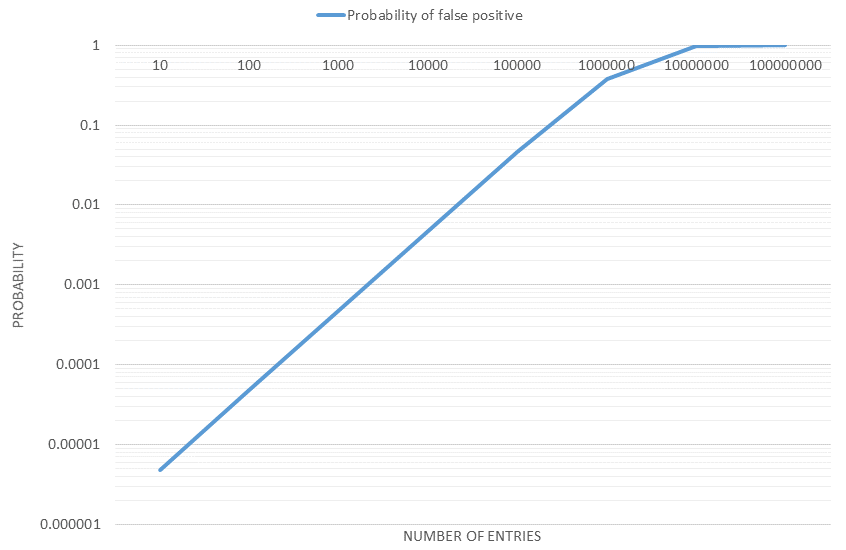
\includegraphics[scale=0.5]{Images/chart.png}
\caption{Name your figure}
\label{chart}
\end{figure}

\subsection{Motivation}

A paragraph for motivation.

\subsection{Objective}

give objective in bulletin.

\begin{enumerate}[i]
\item  to done a through survey on XXXXXXXXXXXXXXXXXXXXX.
\item to develope XXXXXXXXXXXXXXXXXXXXX.
\item to reduce computational time by XXXXXXXXXXXXXXXXXXXXX.
\end{enumerate}



\cite{Oldham:74}\cite{Monje:10}\cite{Miller:93}\cite{Shantanu:11,podlunbybook:90}
\fancyhead[RE]{\fontsize{8}{12}\selectfont\uppercase{Introduction}}
	 % Introduction
\fancyhead[RE]{\fontsize{8}{12}\selectfont\leftmark}
\chapter{Literature survey}
\label{survey}

This id the format for table:



\begin{table}[ht]
\caption{Table Name}
\centering
\begin{tabular}{cc|c|c|c|c|l}
\cline{3-6}
& & \multicolumn{4}{ c| }{Primes} \\ \cline{3-6}
& & 2 & 3 & 5 & 7 \\ \cline{1-6}
\multicolumn{1}{ |c  }{\multirow{2}{*}{Powers} } &
\multicolumn{1}{ |c| }{504} & 3 & 2 & 0 & 1 &     \\ \cline{2-6}
\multicolumn{1}{ |c  }{}                        &
\multicolumn{1}{ |c| }{540} & 2 & 3 & 1 & 0 &     \\ \cline{1-6}
\multicolumn{1}{ |c  }{\multirow{2}{*}{Powers} } &
\multicolumn{1}{ |c| }{gcd} & 2 & 2 & 0 & 0 & min \\ \cline{2-6}
\multicolumn{1}{ |c  }{}                        &
\multicolumn{1}{ |c| }{lcm} & 3 & 3 & 1 & 1 & max \\ \cline{1-6}
\end{tabular}
\label{tab}
\end{table}










 % Literature Review 
\fancyhead[RE]{\fontsize{8}{12}\selectfont\leftmark}
\chapter{Proposed System}
\label{pwork}



\begin{algorithm}[H]
\caption{Your Algorithm Name}
\begin{algorithmic}[1]
\Procedure{Foo}{$Array[],~n$}
	\State $i\leftarrow 0$
    \If{$n\neq 0$}
    	\State $Positive$
    \Else
    	\State $Negative$
     \EndIf
     \For{$i\leftarrow 1~to~n$}
     	\State $Print~Array[i]$
     \EndFor
\EndProcedure
\end{algorithmic}
\end{algorithm}








	 % Level Control in Two-Tank
\fancyhead[RE]{\fontsize{8}{12}\selectfont\leftmark}
\chapter{Experimental Results and Discussions}
\label{pwork1}


This chapter is for experimental results and discussions.












 % QTP
%\fancyhead[RE]{\fontsize{8}{12}\selectfont\leftmark}
\chapter{Your Propose Work 2}
\label{pwork2}







 % Maglev/BP
%\fancyhead[RE]{\fontsize{8}{12}\selectfont\leftmark}
\chapter{Your Propose work 3}
\label{pwork3}











 % FOQFT
\fancyhead[RE]{\fontsize{8}{12}\selectfont\leftmark}
\chapter{Conclusion and Future Work}
\label{DFC}


This is Conclusion chapter.








 % Conclusions
%% ----------------------------------------------------------------
% Now begin the Appendices, including them as separate files

%\addtocontents{toc}{\vspace{1em}}
\backmatter
%\setstretch{1.0}
\setstretch{1.0}
% Add a gap in the Contents, for aesthetics
%\chapter{Publication from the thesis}

1. Conference..\\
2. Journal/Transaction\\
3. Book Chapter\\
4. Etc.
%\appendix % Cue to tell LaTeX that the following 'chapters' are Appendices

\addcontentsline{toc}{chapter}{References}
\bibliographystyle{ieeetr}
\bibliography{mybibfile}

%\chapter{An Appendix}

Appendices are not important to understand the thesis, but improve the quality of the thesis.	% Appendix Title
%\chapter{Publication from the thesis}

1. Conference..\\
2. Journal/Transaction\\
3. Book Chapter\\
4. Etc. % Appendix Title

%\input{Appendices/AppendixC} % Appendix Title

%% For Index
%\printindex


\end{document}  % The End
%% ----------------------------------------------------------------